\section{Requerimientos no funcionales} \label{reqnofuncional}
Se ha realizado una breve revisión de las tecnologías y abordajes brindadas como requerimientos funcionales. Sin embargo, al utilizar un abordaje ágil, la validación de las decisiones tecnológicas depende en ultima instancia de la validación del proceso de desarrollo realizada por expertos y usuarios.

Las decisiones de tecnologías para el módulo de gestión curricular fueron basadas en los conocimientos adquiridos de los miembros del equipo de desarrollo, con el fin de optimizar tiempos utilizados en curvas de aprendizaje. Sin embargo, se hicieron análisis previos a su uso para corroborar que dichas tecnologías cumplen con el propósito de desarrollo.

En las siguientes secciones estaremos describiendo algunas de las tecnologías utilizadas.

\subsection{Java}
La elección del lenguaje de programación, establecida por la organización, fue utilizada como lenguaje para la lógica del módulo curricular ya que facilita su mantenimiento por parte del equipo de desarrolladores. El equipo de desarrollo posee conocimiento en este lenguaje de programación o en lenguajes orientados a objetos, por lo que se aprovechó el tiempo que pudo haber sido utilizado en curvas de aprendizaje del lenguaje para investigar buenas prácticas para el proyecto.

Java fue diseñado para alcanzar los desafíos del desarrollo de aplicaciones en el contexto de ambientes heterogéneos y distribuidos en red. Lo más importante de solucionar entre estos desafíos era la entrega segura de aplicaciones que consumen lo mínimo de recursos del sistema, correr en cualquier plataforma de hardware y/o software, y que pueda ser extendido de manera dinámica.

Operar en múltiples plataformas con redes heterogéneas invalida la arquitectura tradicional de distribución de binarios, \enquote{release}, actualización, parcheo, etc. Para lograr sobresalir, JAVA se convirtió en una arquitectura neutral, portable y adaptable de manera dinámica.

Hoy día, Java es uno de los lenguajes de programación más utilizados a nivel mundial debido a su portabilidad y evolución con el paso del tiempo. Además, al ser un lenguaje de programación multiplataforma cualquier proyecto se puede desarrollar en cualquier sistema operativo o plataforma para luego ser levantada en el servidor independiente a su plataforma. 

El lenguaje es reconocido por ser intuitivo a la hora de programar, altamente portátil y portable. Además, la comunidad es uno de los fuertes de Java, ya que hay cursos en línea para todos los niveles de conocimiento. Además, en la Web hay una gran cantidad de foros y librerías de la comunidad para resolver diferentes problemáticas de los desarrolladores. En la figura \ref{graph_java} se pueden observar cuáles son los lenguajes de programación más utilizados en la comunidad de desarrolladores en los últimos años.

\begin{figure}[H]
\centering
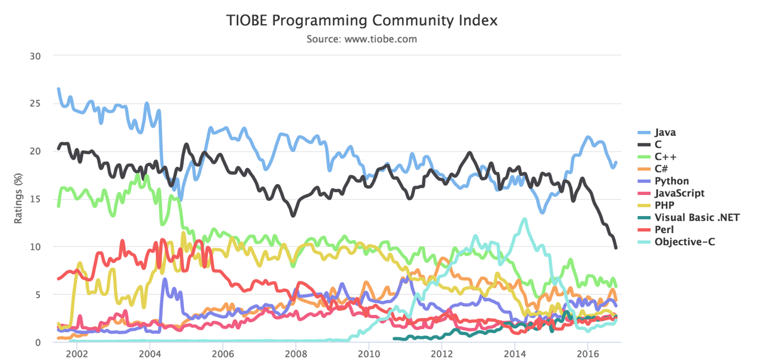
\includegraphics[width=125mm,scale=1]{Figuras/tecnologias/java}
\caption{Gráfico de uso de lenguajes de programación con respecto al tiempo.}
  \label{graph_java}
\end{figure}

Como análisis de posibles riesgos se hizo una breve búsqueda de vulnerabilidades, pero como no hubo riesgos importantes a tener en cuenta se decidió seguir utilizando el lenguaje de programación Java como estuvo previsto. El lenguaje Java proporciona un nivel de rendimiento adecuado para la plataforma donde se aloja el AMS.

Dicho uso del lenguaje fue validado durante el proceso de desarrollo al poder resolver los criterios de aceptación de las historias de usuario.

\subsection{MySQL}
Para ayudar a que el AMS sea adaptable y fácil de mantener, se extenderá la base de datos ya utilizada por el AMS. Por lo tanto, la elección de la base de datos del módulo queda a criterio de la organización y como requisito no funcional para el proyecto final. El sistema de base de datos que se utiliza para el sistema de evaluación de competencias es MySQL, por ser un sistema open source y con una de las comunidades más grandes entre las bases de datos existentes.

MySQL es el sistema de base de datos open source más popular disponible. Es particularmente eficaz para sitios web públicos que requieren base de datos rápidas y estables\citep{dyer2015learning}. Como colección estructurada de datos puede ser utilizada como gestor para cualquier tipo de solución, desde una lista de compras hasta una enorme cantidad de información de una red empresarial. Para añadir, acceder y procesar datos almacenados en una base de datos informática se necesita de un sistema de administración de Base de Datos como MySQL Server. Como las computadoras son muy buenas manejando grandes cantidades de datos, los sistemas de administración de base de datos juegan un rol principal en la computación como utilidades autónomas o como partes de otras aplicaciones.

Para representar los datos que almacena utiliza el modelo lógico de datos relacional donde almacena sus datos en tablas separadas, antes que almacenar todos los datos en un solo lugar. La estructura de la base de datos está organizada en archivos físicos optimizados para mayor velocidad. El modelo lógico con objetos tales como bases de datos, tablas, vistas, filas, y columnas, ofrecen un ambiente de programación flexible donde se establecen reglas que gobiernan las relaciones entre las de los distintos tipos de campos, tales como uno a uno, uno a muchos, únicos, requeridos, u opcionales y punteros entre diferentes tablas.

Hemos utilizado este motor de base de datos en nuestra vida cotidiana sin darnos cuenta; en Google, Amazon, Facebook, Wikipedia y otros sitios web populares. Es el guardián de los datos detrás de grandes sitios con cientas de páginas de datos, sin dejar atrás los pequeños sitios con solo algunas páginas. También es utilizado en aplicaciones que no son basadas en web. Es rápida, estable y pequeña cuando se requiere.

En las siguientes figuras podemos observar que MySQL es un sistema de manejo de base de datos muy utilizado por la comunidad y va en aumento de popularidad hasta casi alcanzar a uno de los gigantes que es Oracle.

\begin{figure}[H]
\centering
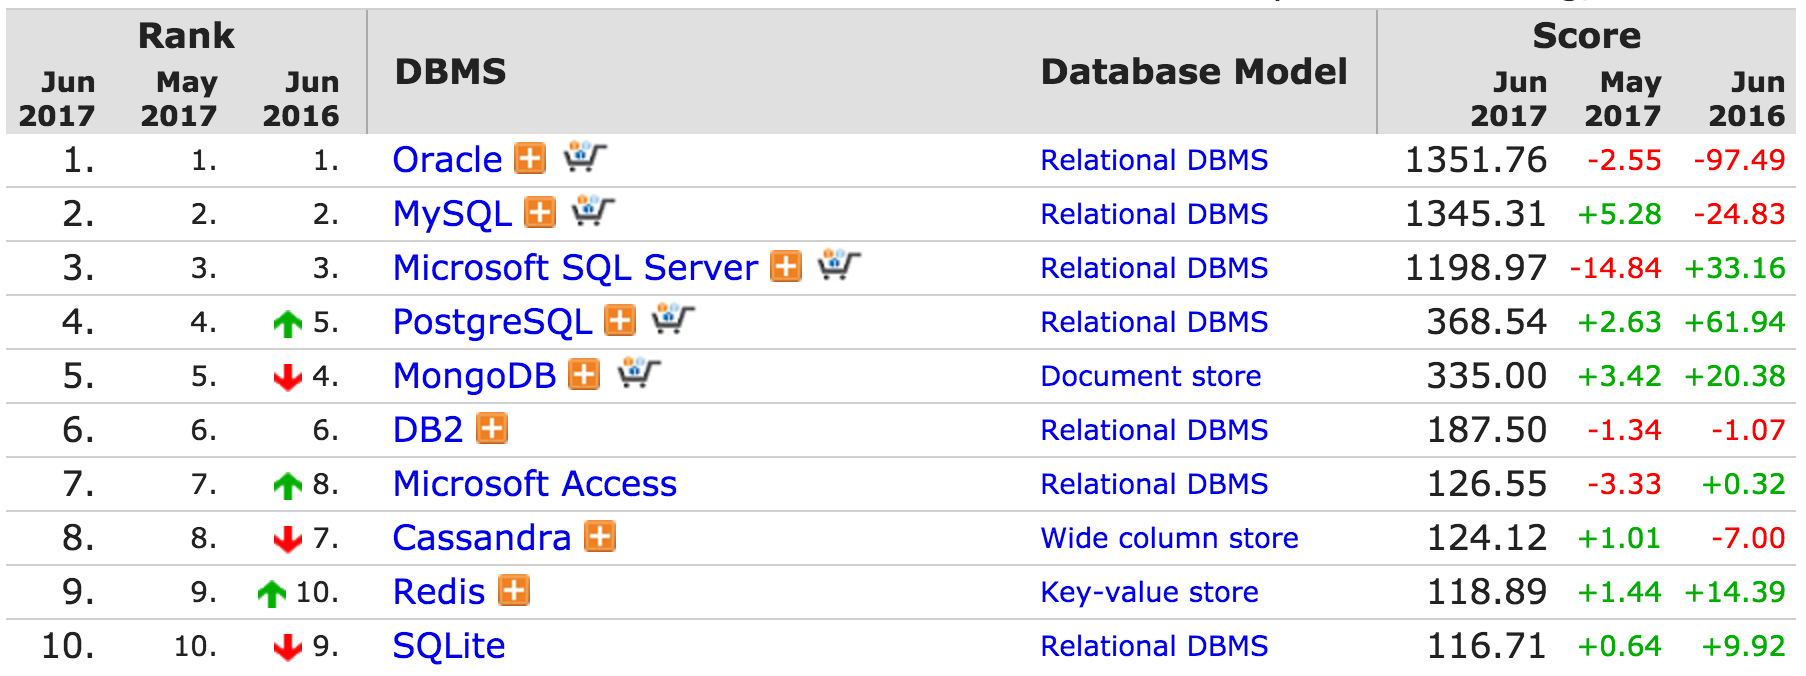
\includegraphics[width=125mm,scale=1]{Figuras/tecnologias/rank_db_1}
% \caption{Gráfico de uso de lenguajes de programación con respecto al tiempo.}
  \label{graph_db_1}
\end{figure}

\begin{figure}[H]
\centering
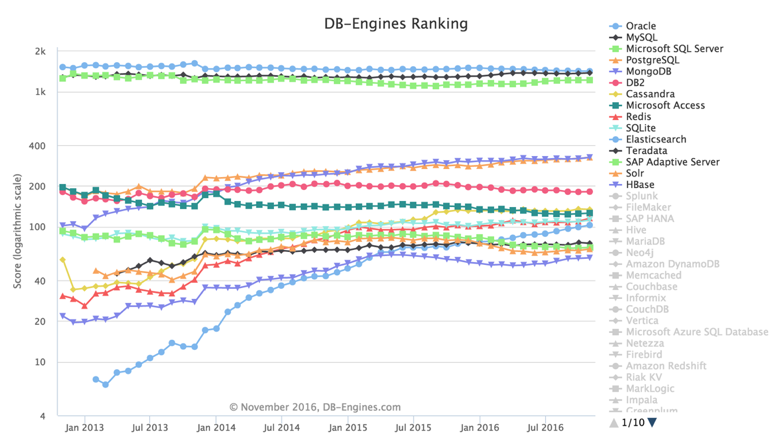
\includegraphics[width=125mm,scale=1]{Figuras/tecnologias/rank_db_2}
\caption{Gráfico de uso de motores de base de datos con respecto al tiempo.}
  \label{graph_db_2}
\end{figure}

Como el motor de base de datos es otro requerimiento no funcional, como es otra tecnología utilizada para la aplicación base. Sin embargo, se hizo un breve análisis de vulnerabilidades para verificar que el uso de MySQL como base de datos relacional podría ser efectivo para el proyecto final pero como no se encontraron vulnerabilidades críticas se continuó el uso de la misma. Además, los desarrolladores están familiarizados con la misma.

\subsection{NoSQL}

\subsection{Amazon Web Services}
Amazon Web Services, o más conocida como AWS, es una plataforma de servicios web que ofrece soluciones de procesado, almacenamiento y redes en diferentes capas de abstracción. Se pueden usar estos servicios para hospedar sitios web, correr aplicaciones complejas y para minería de grandes cantidades de datos. [X] Nos referimos por servicios web a aquellos\ servicios que pueden ser controlados o accedidos por medio de una interfaz web. La interfaz web puede ser manejada por máquinas o por usuarios por medio de una interfaz de usuario gráfica. Los servicios más utilizados son EC2 en la cual ofrece servidores virtuales, y S3 que es utilizada para almacenamiento.

AWS es una nube pública, donde tiene las siguientes clasificaciones como nube:
\begin{itemize}
	\item \textbf{Infraestructura como Servicio:} más conocida como IaaS, ofrece recursos fundamentales como procesamiento, almacenamiento, y capacidades de servicios, utilizando servidores virtuales tales como Amazon EC2, Google Compute Engine y Microsoft Azure en las máquinas virtuales.
	\item \textbf{Plataforma como Servicio:} más conocida como PaaS, provee plataformas para desplegar aplicaciones customizadas a la nube, tales como AWS Elastic Beanstalk, Google App Engine, y Heroku.
	\item \textbf{Software como Servicio:} más conocida como SaaS, combina infraestructura y software corriendo en la nube, incluyendo aplicaciones de oficina como Amazon WorkSpaces, Google Apps for Work, y Microsoft Office 365.
\end{itemize}

En la figura \ref{graph_cloud} AWS se encuentra en la cabecera debido a su buen servicio y ser uno de los primeros de ofrecer servicios de infraestructura como servicio.

\begin{figure}[H]
\centering
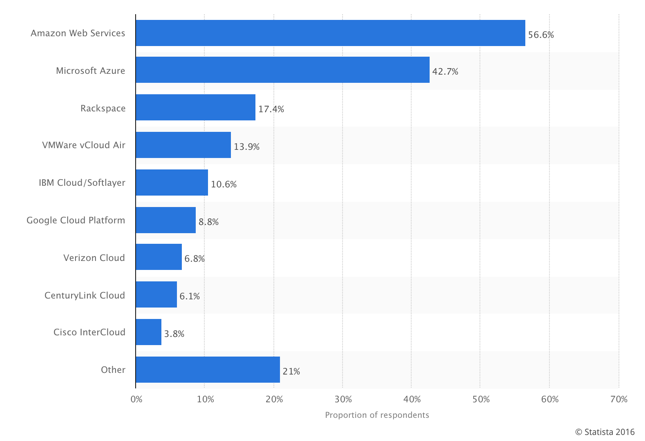
\includegraphics[width=125mm,scale=1]{Figuras/tecnologias/rank_cloud}
\caption{Ranking de compañias que brindan servicios de cloud computing.}
  \label{graph_cloud}
\end{figure}

El AMS se encuentra alojado en la plataforma de servicios AWS. Por lo tanto, se utilizaron los servidores ya en línea para correr el módulo curricular para la aplicación.

\subsection{Git}
Para mejorar la integración del código que produce el equipo, la organización utiliza un repositorio en \enquote{GitHub}\footnote{Plataforma de desarrollo colaborativo de software para alojar proyectos utilizando el sistema de control de versiones Git.} para almacenar el código. Además, el uso de un sistema de versionamiento permite minimizar y optimizar el tiempo de unión de módulos que van agregando o actualizando los miembros del equipo de desarrollo. Por lo tanto, un trabajo en equipo requiere de un sistema de control de versiones eficiente. Partiremos explicando los conceptos relativos a las herramientas de control de versiones.

El control de versiones es un sistema que registra los cambios realizados sobre un archivo o conjunto de archivos a lo largo del tiempo, de esta forma permite recuperar versiones específicas más adelante. [X]

Git modela sus datos más como un conjunto de instantáneas de un pequeño sistema de archivos. Cada vez que se confirma el cambio de un archivo, o se guarda el estado de un proyecto se hace una foto del aspecto de todos los archivos en ese momento y guarda una referencia a esa instantánea. Para ser eficiente, si los archivos no se han modificado, Git no almacena el archivo de nuevo, solo un enlace al archivo idéntico anterior que ya tiene almacenado. Tiene un comportamiento como en el siguiente gráfico. 

\begin{figure}[H]
\centering
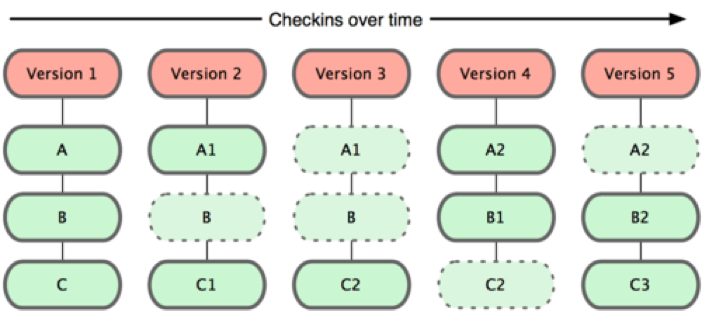
\includegraphics[width=125mm,scale=1]{Figuras/tecnologias/git_over_time}
\caption{Flujo de versiones de Git.}
  \label{graph_git}
\end{figure}

Uno de los fuertes importantes de Git como VCS\footnote{de sus siglas en inglés, Version Control System, que significa en español sistema de control de versionamiento.} es su integridad, debido a que toda versión es verificada mediante una suma de comprobación\footnote{También conocida como checksum.} antes de ser almacenado, y es identificado a partir de ese momento dicha suma. Esta suma es utilizada para volver a un estado anterior del repositorio en caso de ser necesario o ver cuáles fueron los cambios que se realizaron en ese pedazo de código trabajado o más conocido como commit.

\subsection{Spring}
El AMS cuenta con un framework deprecado y uno nuevo en el cuál se estuvo trabajando para los nuevos módulos que se fueron desarrollando, donde entra el uso de Spring MVC como framework para la parte lógica de la aplicación, por lo que requiere un estudio de la documentación que ofrece Spring para empezar a utilizar el framework y de las buenas practicas establecidas por el equipo de desarrollo.

Spring es un framework que facilita el desarrollo de aplicaciones escritas en Java. El propósito de Spring es manejar la infraestructura de las aplicaciones y el programador sólo se centre en la aplicación. Es por ello, que el programador se encargará de programar la lógica de negocio usando objetos simples de Java o POJOs (Plain Old Java Objets) y Spring se encargará de añadir las capacidades de empresa o J2EE a nuestra aplicación. [X]

Spring tiene las siguientes características:
\begin{itemize}
	\item Simplicidad y acoplamiento débil donde permite programar Java de manera sencilla. Busca ser simple y se basa en la inyección de dependencias para obtener un acoplamiento débil.
	\item Funciona como contenedor ya que gestiona el ciclo de vida de los objetos y como se relacionan entre ellos. Proporciona una gran infraestructura que permite que el programador se dedique a la lógica de la aplicación.
	\item Ligero porque es muy rápido en tiempo de procesamiento y no es invasivo a la hora de programar.
	\item Orientado a aspectos ya que soporta la programación orientada a aspectos, lo que permite facilitar una capa de servicios que son ideales para este tipo de programación como auditoría, o gestión de transacciones.
\end{itemize} 

Spring se utiliza en el proyecto como framework para toda la aplicación, por lo tanto, usar Spring es también un requerimiento no funcional.

\subsection{AngularJS}
Para empezar a trabajar con la interfaz de usuario se hizo un estudio previo de las ventajas entre Frameworks como JQuery y AngularJS, debido a que la organización que brinda el AMS dio total libertad a la hora de elegir cual utilizar. Por lo tanto, la elección del framework Javascript del módulo de Curriculum entra como decisión de diseño para el proyecto final.  Por lo tanto, es relevante explicar brevemente la historia de los diferentes frameworks de Javascript para poder comprender las mejoras que tuvo la misma a lo largo del tiempo.

Con la llegada de los framework de Javascript, tales como JQuery, las páginas web ya no tenían la necesidad de volver a renderizar las páginas cada vez que se necesitaba información del servidor, ya que con la aparición de las llamadas asíncronas se ha logrado mejorar la experiencia del usuario.

JQuery ha hecho un excepcional trabajo al proveer de herramientas que manipulen el DOM de una página, pero no ofrece una guía real de cómo organizar el código en la estructura de la aplicación. Ante la desesperada búsqueda de escribir aplicaciones grandes y fáciles de mantener en Javascript ha dado a luz a un renacimiento de Frameworks de Javascript, entre ellos se encuentra el framework de Google más conocida como AngularJS.

AngularJS es un framework de aplicaciones web de código abierto que ofrece a un desarrollador una base estable de código con una comunidad enorme y un entorno rico de librerías hechas por la comunidad.